\documentclass[11pt,letterpaper]{article}
\usepackage[lmargin=1in,rmargin=1in,tmargin=1in,bmargin=1in]{geometry}
\usepackage{../style/homework}
\usepackage{../style/commands}
\setbool{quotetype}{false} % True: Side; False: Under
\setbool{hideans}{true} % Student: True; Instructor: False

\newcommand{\blank}[1]{\underline{\hspace{#1}}} % Blank Underline

% -------------------
% Content
% -------------------
\begin{document}

\homework{17: Due 12/12}{Geometric diagrams are to geometers what board and pieces are to chess masters: visual aids, helpful but not indispensable.}{Richard J. Trudeau}

% Problem 1
\problem{10} Consider the graph $G$ given below.
	\begin{figure}[h]
	\centering
	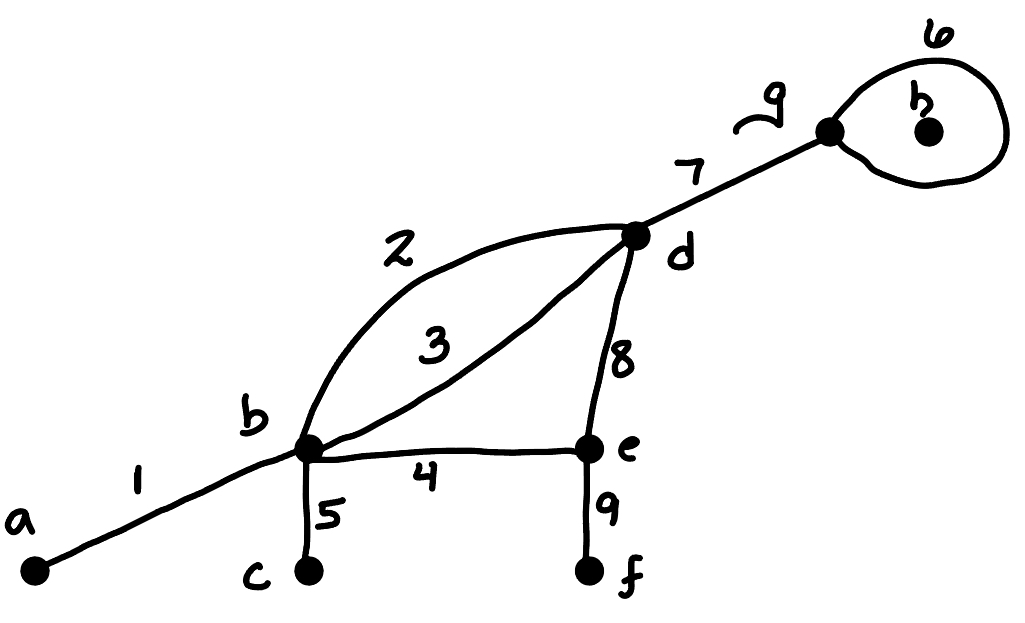
\includegraphics[width=0.3\textwidth]{graph1.jpg}
	\end{figure}

\begin{2enumerate}
\item Is $b$ adjacent to $f$? Explain.
\item Are $4$ and $8$ parallel? Explain. 
\item Are there isolated vertices? Explain.
\item Is the graph simple? Explain. 
\item Is the graph connected? Explain. 
\item What are the endpoints of $5$?
\item is $g$ incident to $3$? Explain. 
\item What is $\deg(g)$?
\item What is $\deg(b)$?
\item What is the degree of $G$?
\end{2enumerate}




\newpage



% Problem 2
\problem{10} Being sure to show all your work and fully justify your answers, complete the following:
	\begin{enumerate}[(a)]
	\item Draw a simple graph with three vertices that has a unique isolated vertex. 
	\item Draw the graph $K_6$. 
	\item Draw the graph $K_{5, 2}$. 
	\item Draw the undirected graph given by the following adjacency matrix:
		\[
		\begin{pmatrix}
		1 & 1 & 0 & 0 & 1 \\
		1 & 0 & 1 & 0 & 0 \\
		0 & 1 & 0 & 2 & 0 \\
		0 & 0 & 2 & 0 & 1 \\
		1 & 0 & 0 & 1 & 0 
		\end{pmatrix}
		\]
	\end{enumerate}



\newpage



% Problem 3
\problem{10} Consider the graph $G$ below.
	\begin{figure}[h]
	\centering
	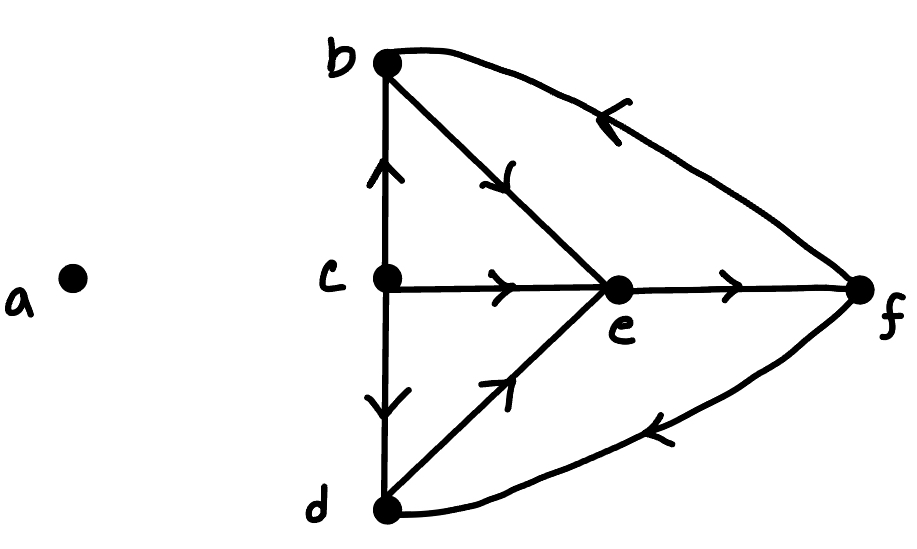
\includegraphics[width=0.3\textwidth]{graph2.jpg}
	\end{figure}
\begin{enumerate}[(a)]
\item Is $e$ adjacent to $c$? Explain. Is $c$ adjacent to $e$? Explain. 
\item Find the adjacency matrix of the graph.
\item Find the in and out degree of each vertex. 
\item Does $G$ have any sources or sinks? Explain. 
\end{enumerate}



\newpage



% Problem 4
\problem{10} The adjacency matrix for an undirected graph $G$ is given below. 
	\[
	\begin{pmatrix}
	0 & 1 & 0 & 0 & 0 & 0 & 0 \\
	1 & 0 & 2 & 0 & 0 & 0 & 0 \\
	0 & 2 & 0 & 1 & 0 & 0 & 0 \\
	0 & 0 & 1 & 0 & 0 & 0 & 0 \\
	0 & 0 & 0 & 0 & 0 & 0 & 0 \\
	0 & 0 & 0 & 0 & 0 & 1 & 1 \\
	0 & 0 & 0 & 0 & 0 & 1 & 1 \\
	\end{pmatrix}
	\]

\begin{enumerate}[(a)]
\item Find $|V(G)|$ and $|E(G)|$. 
\item Are there any loops in $G$? Explain. 
\item Does $G$ have parallel edges? Explain.
\item Find the degree of $G$. 
\item How many connected components does $G$ have? Explain. 
\end{enumerate}


\end{document}